\documentclass[tikz,border=10pt]{standalone}
\usepackage{fontspec}
\setmainfont{IBM Plex Serif}
\usepackage{unicode-math}
\setmathfont{STIX Two Math}
\usepackage{pgfplots}
\pgfplotsset{compat=newest}
\begin{document}
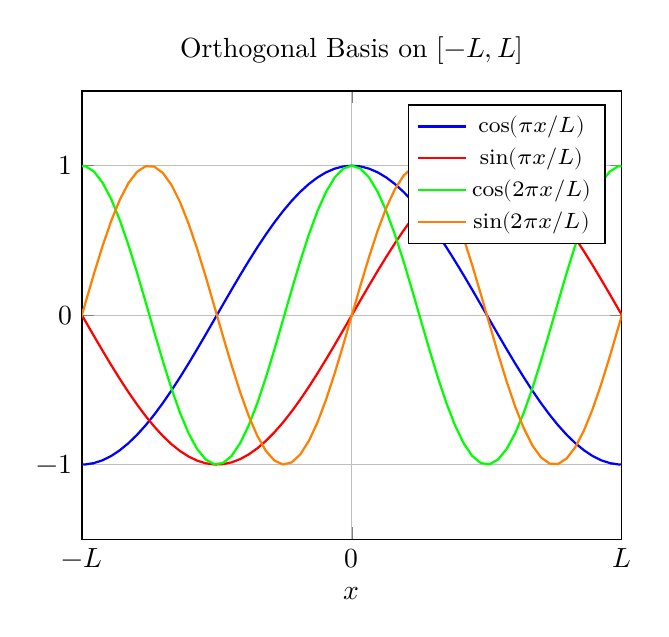
\begin{tikzpicture}
    \begin{axis}[
            xlabel={\(x\)},
            ylabel={},
            title={Orthogonal Basis on \([-L,L]\)},
            xmin=-3.14, xmax=3.14,
            ymin=-1.5, ymax=1.5,
            grid=major,
            legend pos=north east,
            samples=101,
            xtick={-3.14, 0, 3.14},
            xticklabels={\(-L\), \(0\), \(L\)},
            legend style={font=\footnotesize}
        ]

        % Show orthogonal basis functions
        \addplot[blue, thick] {cos(deg(x))};
        \addlegendentry{\(\cos(\pi x/L)\)}

        \addplot[red, thick] {sin(deg(x))};
        \addlegendentry{\(\sin(\pi x/L)\)}

        \addplot[green, thick] {cos(deg(2*x))};
        \addlegendentry{\(\cos(2\pi x/L)\)}

        \addplot[orange, thick] {sin(deg(2*x))};
        \addlegendentry{\(\sin(2\pi x/L)\)}

    \end{axis}
\end{tikzpicture}
\end{document}
